% A short description of our team members
% I will add the outline of my description, just copy and paste it over and add your details -> also keep it aplhabetically -> see readMe for order of members

%start of member section
%WITHOUT STUFF THERE IS CHAOS :P 
\subsection{Elzahn Botha}
\begin{wrapfigure}[6]{l}{90px}

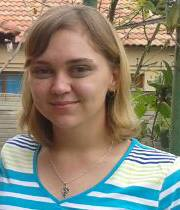
\includegraphics[width=80px]{ElzahnBotha.jpg}
\end{wrapfigure}

\textcolor{white}{.}
\subsubsection{Interests}
\begin{itemize}
	\item[-]{Video Games}
	\item[-]{Game development}
	\item[-]{Programming}
	\item[-]{Anime}
\end{itemize}
\subsubsection{Technical Skills} 
\begin{itemize}
	\item[-]{I have already been exposed to Java and been working with it for about a year now}
\end{itemize}
\subsubsection{Past Experience}
\begin{itemize}
	\item[-]{I have experience in writing programs and systems in Java}
\end{itemize}
\subsubsection{Non-Technical Strengths} 
\begin{itemize}
	\item[-]{Hard and dedicated worker}
	\item[-]{Always ready to learn new technologies and languages}
	\item[-]{Functions best under pressure}
\end{itemize}
\subsubsection{Why I want to do this project}
This project seemed like it would be a rather interesting project to do as well as the fact that it would be great exposure to a whole new side of IT that I have not yet had the privilege of delving into. I believe that by doing this project I will get valuable exposure that can later help in other projects that I might attempt. This project also seems like it would be a good challenge since I am more comfortable with smaller projects and systems and by doing a larger project such as this it will help me broaden my range of capabilities. Lastly due to the size of the project and the strict time line the pressure will be greatly increased helping me to work at my best without losing interest with the project. 

\pagebreak
\subsection{Jason Richard Evans}
\begin{wrapfigure}[5]{l}{100px}
\vspace{10pt}

\includegraphics[width=80px]{Jason.jpg}
\end{wrapfigure}

\textcolor{white}{.}
\subsubsection{Interests}
\begin{itemize}
	\item{Music Enthusiast}
	\item{Software development}
	\item{Adventure Sports}
\end{itemize}
\subsubsection{Technical Skills}
\begin{itemize}
	\item{C++ and Java}
	\item{Web Development}
\end{itemize}
\subsubsection{Past Experience}
%WHAT SHOULD I WRITE HERE??
Assignments and projects completed for University purposes. A lot of exposure with writing Java applications and servers.
\subsubsection{Non-Technical Strengths}
\begin{itemize}
	\item{Positive outlook on life}
	\item{Hard worker}
	\item{Good team worker}
	\item{An eager learner}
\end{itemize}
\subsubsection{Why I want to do this project}
The reason I started with software development is to make life a bit easier for everyone, and this project fits right into that goal. Creating a software product to teach others an important part of computer science logic more easily and austhetically pleasing will help thousands of students.

\pagebreak
\subsection{Renette Ros}
\begin{wrapfigure}[8]{l}{90px}
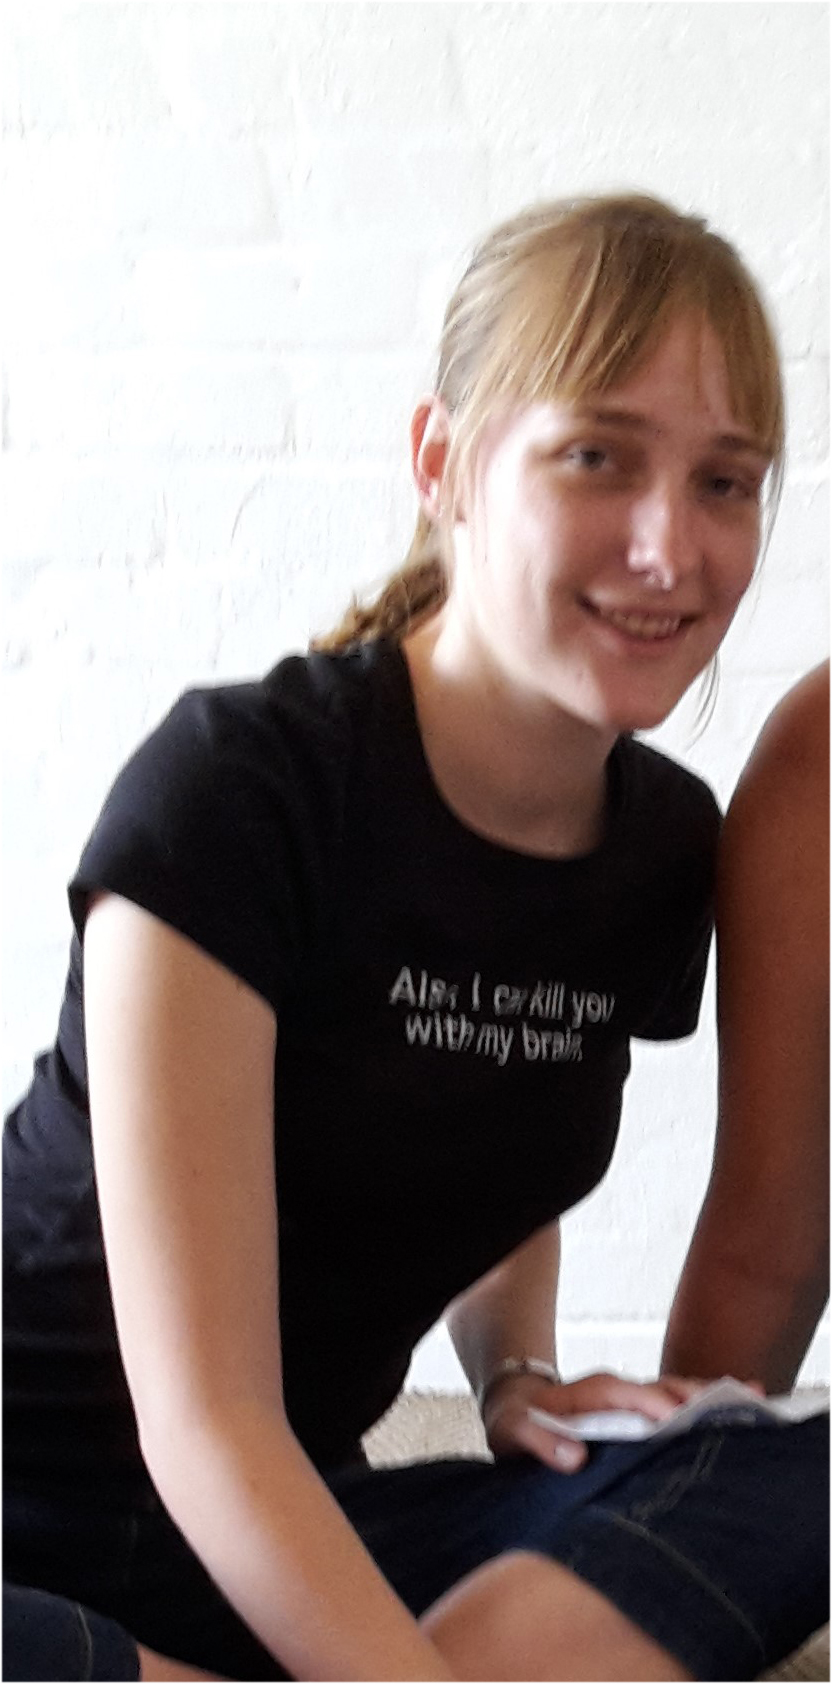
\includegraphics[width=80px]{Renette.jpg}
\end{wrapfigure}
\textcolor{white}{}
\subsubsection{Interests}
\begin{itemize}
	\item Reading
	\item Playing Games
	\item Painting
	\item Puzzles and problem solving
	\item Programming
	\item New interesting technologies
\end{itemize}
\subsubsection{Technical Skills}
\begin{itemize}
	\item Java
	\item C++
	\item Web Development
	\item HCI - User Experience and User interface design
	\item XML, XML Schemas and related technologies.
	\item Good at identifying possible problems and debugging code
\end{itemize}
%\subsubsection{Past Experience}

\subsubsection{Non-Technical Strengths}
\begin{itemize}
	\item Hard Worker
	\item I don't like to do things halfway
	\item I learn new technologies easily
	\item I'm very enthusiastic about things I'm interested in.
\end{itemize}
\subsubsection{Why I want to do this project}
I want to do this project because creating an application like this will be very interesting because it is completely different from the things we have done up to now. I also believe it is important to have flowcharting software that forces students to create correctly structured flowcharts but is still easy to use since I got frustrated a lot with the flowcharting software we used in COS151.

\pagebreak
\subsection{Szymon Ziolkowski}
\begin{wrapfigure}[5]{l}{100px}
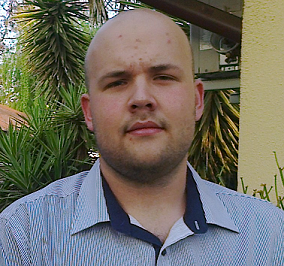
\includegraphics[width=80px]{Szymon.png}
\end{wrapfigure}

\textcolor{white}{.}
\subsubsection{Interests}
	\begin{itemize}
		\item Networks
		\item Security
		\item Computer hardware and electronics
		\item Paintball
		\item Video games
	\end{itemize}
\subsubsection{Technical Skills} 
	\begin{itemize}
		\item C\# and Java
		\item Web development
		\item SQLite, MySQL and SQL Server
	\end{itemize}
	
\subsubsection{Past Experience}
I have no past experience that might be relevant to the project. %dont forget to remove this%
\subsubsection{Non-Technical Strengths}
	\begin{itemize}
		\item Don't give up easily
		\item Helpful
	\end{itemize}
\subsubsection{Why I want to do this project} 

\pagebreak
\subsection{Vivian Laura-Lee Venter}
\begin{wrapfigure}[7]{l}{150px}
\vspace{10pt}

\includegraphics[width=150px]{Vivian.png}
\end{wrapfigure}

\textcolor{white}{.}
\subsubsection{Interests}
\begin{itemize}
	\item{Computer Games}
		\subitem- First Person Shooter
		\subitem- Sport/Soccer
		\subitem- Strategic
	\item{Music And Movies}
	\item{Watching Sports Fanatic: }
		\subitem -Rugby 
		\subitem -Football
		\subitem -Cricket
		\subitem -Athletics
	\item{Software Development/Programming}
	\item{Computer Hardware/Gaming System builds Fanatic }
\end{itemize}
\subsubsection{Technical Skills}
\begin{itemize}
	\item{Java and JavaFX}
	\item{C++}
	\item{Client/Server Applications (Beginner)}
	\item{Web Development (Beginner)}
	\item{Design Patterns}
	\item{Program/System Tester and Debugging}
\end{itemize}

\subsubsection{Non-Technical Strengths}
\begin{itemize}
	\item{Hard-Worker}
	\item{Compationate}
	\item{Competent in knowledgeable/experienced fields}
	\item{Good Listener}
	\item{Diligent}
	\item{Integrity}
	\item{Willing and keen Learner}
	\item{Dedicated to my studies and work}
	\item{Team Player}
	\item{Leader when I need to be}
\end{itemize}
\subsubsection{Past Experience} 
\begin{itemize}
	\item{I have written Java programs and small systems as assignments for my modules at the University of Pretoria}
	\item{I have written C++ programs and small systems as assignments for my modules at the University of Pretoria}
	\item{I have written several types of server programs (e.g HTTP) as assignments for my modules at the University of Pretoria}
\end{itemize}
\subsubsection{Why I want to do this project}
Stuff
%end of member section